\documentclass[tikz,11pt]{{standalone}} 
%%%<
\usepackage{verbatim}


\begin{document}

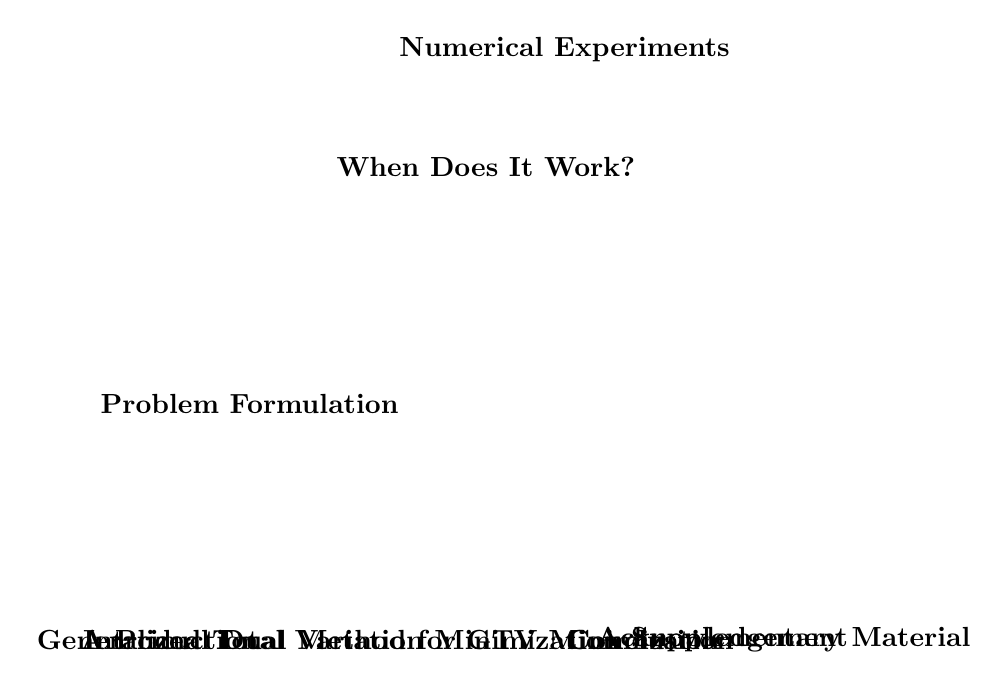
\begin{tikzpicture}[x=0.5cm,y=1.5cm]
\node (Introduction) at (0, 0) {\textbf{Introduction}};
\node (Problem_Formulation) at (2, 2) {\textbf{Problem Formulation}};
\node (Generalized_Total_Variation_Minimization) at (4, 0) {\textbf{Generalized Total Variation Minimization}};
\node (A_Primal_Dual_Method_for_GTV_Minimization) at (6, 0) {\textbf{A Primal Dual Method for GTV Minimization}};
\node (When_Does_It_Work?) at (8, 4) {\textbf{When Does It Work?}};
\node (Numerical_Experiments) at (10,5) {\textbf{Numerical Experiments}};
\node (Conclusion) at (12, 0) {\textbf{Conclusion}};
\node (Acknowledgement) at (14, 0) {\textbf{Acknowledgement}};
\node (Supplementary_Material) at (16, 0) {\textbf{Supplementary Material}};
\end{tikzpicture}
\end{document} 